\documentclass{article}
\usepackage{amsmath, amssymb, array, enumerate, tikz, multicol, hyperref, sfmath, pgfplots, tcolorbox}
\pgfplotsset{compat = newest}
\renewcommand{\familydefault}{\sfdefault}
\usepackage[top = 0.5in, bottom=0.5in, right = 1in, left = 1in]{geometry}
\tikzset{>=stealth}
\pagestyle{empty}
\raggedright

\newcounter{example}[section]
\newenvironment{example}[1][]{\refstepcounter{example}\par\medskip
   {\color{red}\textbf{Example~\theexample. #1}}}{\medskip}

\begin{document}

\section*{Factoring Special Forms}

\begin{tcolorbox}[colframe=orange!70!white, coltitle=black, title=\textbf{Summary}]
\begin{enumerate}
    \item Always look for a greatest common factor (GCF) to factor out \emph{first}.
    \item $a^3 + b^3 = (a+b)(a^2 - ab + b^2)$
    \item $a^3 - b^3 = (a-b)(a^2 + ab + b^2)$
\end{enumerate}
\end{tcolorbox}

\subsection*{Factoring Sum of Cubes}

A {\color{blue}\textbf{sum of cubes}} is an expression in the form

\[ a^3 + b^3 \]

To start, take the cube root of each term:
\begin{itemize}
    \item $\sqrt[3]{a^3} = a$
    \item $\sqrt[3]{b^3} = b$
\end{itemize}
\bigskip 

\begin{center}
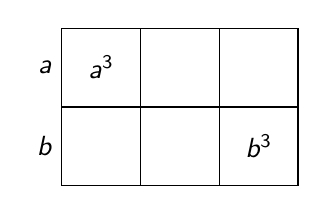
\begin{tikzpicture}
    \draw[black] (0,0) grid (3,2);
    \node at (0,0.5) [left] {$b$};
    \node at (0,1.5) [left] {$a$};
    \node at (0.5,1.5) {$a^3$};
    \node at (2.5,0.5) {$b^3$};
\end{tikzpicture}
\end{center}
\vspace{0.5in} 

\emph{Remember}: Always check to see if you are able to factor out a GCF first.
\bigskip 

\begin{example}
Factor each completely.
\begin{enumerate}[(a)]
\begin{multicols}{3}
    \item $x^3 + 125$
    \item $27y^3 + 64$
    \item $2x^3 + 54$
\end{multicols}
\end{enumerate}
\end{example}

\newpage 

\subsection*{Factoring Difference of Cubes}

A {\color{blue}\textbf{difference of cubes}} is an expression in the form

\[ a^3 - b^3 \]

To start, take the cube root of each term:
\begin{itemize}
    \item $\sqrt[3]{a^3} = a$
    \item $\sqrt[3]{-b^3} = -b$
\end{itemize}
\bigskip 

\begin{center}
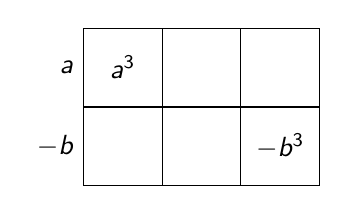
\begin{tikzpicture}
    \draw[black] (0,0) grid (3,2);
    \node at (0,0.5) [left] {$-b$};
    \node at (0,1.5) [left] {$a$};
    \node at (0.5,1.5) {$a^3$};
    \node at (2.5,0.5) {$-b^3$};
\end{tikzpicture}
\end{center}
\vspace{0.5in} 
\bigskip 

\begin{example}
Factor each completely.
\begin{enumerate}[(a)]
\begin{multicols}{3}
    \item $x^3 - 216$
    \item $8 - 125y^3$
    \item $5x^3 - 40$
\end{multicols}
\end{enumerate}
\end{example}

\end{document}
